\documentclass[aspectratio=169,10pt]{beamer}
\usetheme{Madrid}
\usecolortheme{seahorse}
\usepackage[T1]{fontenc}
\usepackage{lmodern}
\usepackage{tikz}
\usetikzlibrary{arrows.meta,positioning,shapes.geometric}
\usepackage{booktabs}
\setbeamertemplate{navigation symbols}{}
\setbeamertemplate{footline}[frame number]
\setbeamercolor{structure}{fg=teal!65!black}
\setbeamercolor{frametitle}{fg=teal!45!black}
\title[MEDORA]{MEDORA}
\subtitle{Integrated Clinic Management and Electronic Medical Records}
\author[Group 08]{System Design -- Group 08}
\institute{Hanoi University of Science and Technology}
\date{2026}

\begin{document}

\begin{frame}[plain]
  \titlepage
  \vspace{-0.5em}
  \centering\small Report review and system concept
\end{frame}

\begin{frame}{The outpatient workflow problem}
  \begin{columns}[T,onlytextwidth]
    \column{.53\textwidth}
      \begin{block}{Need}
        Clinic work spans registration, scheduling, queues, clinical notes, services and payment. Fragmented records and handoffs make the patient journey harder to coordinate and audit.
      \end{block}
      \begin{block}{MEDORA's focus}
        One shared patient identity and encounter record, with explicit workflow states and role-based access.
      \end{block}
    \column{.43\textwidth}
      \centering
      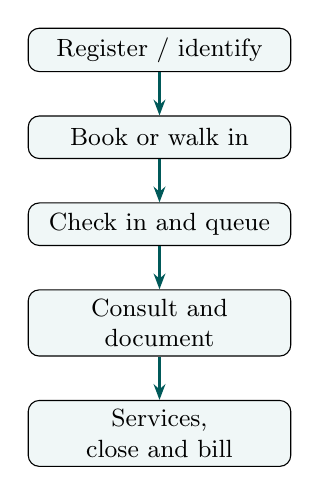
\begin{tikzpicture}[node distance=0.55cm, every node/.style={draw,rounded corners,fill=teal!6,align=center,text width=3.1cm,minimum height=.54cm,font=\small}, arrow/.style={-{Stealth[length=2mm]},thick,teal!70!black}]
        \node (a) {Register / identify};
        \node[below=of a] (b) {Book or walk in};
        \node[below=of b] (c) {Check in and queue};
        \node[below=of c] (d) {Consult and document};
        \node[below=of d] (e) {Services, close and bill};
        \draw[arrow] (a)--(b); \draw[arrow] (b)--(c); \draw[arrow] (c)--(d); \draw[arrow] (d)--(e);
      \end{tikzpicture}
  \end{columns}
\end{frame}

\begin{frame}{System boundary and users}
  \begin{columns}[T,onlytextwidth]
    \column{.5\textwidth}
      \textbf{In scope}
      \begin{itemize}\item Patient identity and longitudinal history
        \item Appointments, walk-ins, check-in and queues
        \item Screening, consultation, notes and prescriptions
        \item Service orders, execution, invoices and payments
        \item Reporting, audit trail and role/scope controls
      \end{itemize}
    \column{.46\textwidth}
      \textbf{Role boundaries}
      \begin{itemize}\item Reception: identity, appointments, queues
        \item Nurse / doctor: screening and clinical decisions
        \item Technician / medicine staff: record service execution
        \item Cashier / finance: payments / authorized refunds
        \item Manager, admin and auditor: oversight and governance
      \end{itemize}
  \end{columns}
  \vspace{.3em}\footnotesize Patient self-service, insurer settlement, external diagnostic systems and advanced inventory are later-stage extensions.
\end{frame}

\begin{frame}{Core design: keep events and records distinct}
  \centering
  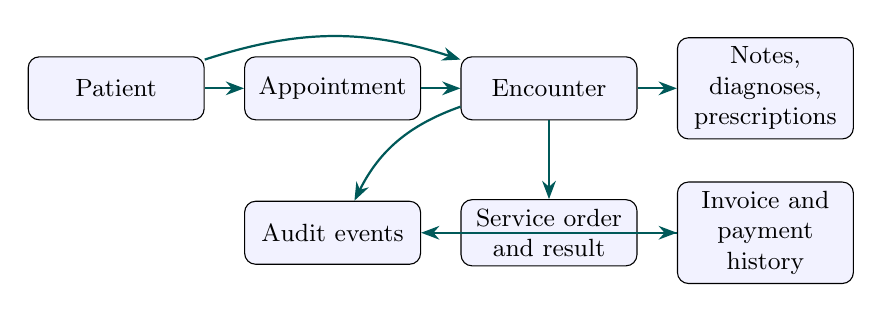
\begin{tikzpicture}[node distance=.55cm and .5cm, box/.style={draw,rounded corners,fill=blue!5,minimum height=.8cm,text width=2.0cm,align=center,font=\small}, arr/.style={-{Stealth},thick,teal!70!black}]
    \node[box] (p) {Patient};
    \node[box,right=of p] (appt) {Appointment};
    \node[box,right=of appt] (enc) {Encounter};
    \node[box,right=of enc] (clin) {Notes, diagnoses, prescriptions};
    \node[box,below=1.0cm of enc] (svc) {Service order and result};
    \node[box,right=of svc] (inv) {Invoice and payment history};
    \node[box,left=of svc] (audit) {Audit events};
    \draw[arr] (p)--(appt); \draw[arr] (p) to[bend left=18] (enc); \draw[arr] (appt)--(enc); \draw[arr] (enc)--(clin);
    \draw[arr] (enc)--(svc); \draw[arr] (svc)--(inv); \draw[arr] (enc) to[bend right=22] (audit); \draw[arr] (inv)--(audit);
  \end{tikzpicture}
  \vspace{1em}
  \begin{block}{Integrity rules emphasized in the report}
    A prescription is not a dispensing event; an order is not a result; signed notes are amended with a reason; refunds append a separate, authorized transaction.
  \end{block}
\end{frame}

\begin{frame}{Requirements and proposed acceptance targets}
  \begin{itemize}
    \item Conflict-free booking under concurrent requests; no duplicate active encounter.
    \item Server-side authorization by role, facility scope and workflow state.
    \item Preserve signed clinical history; require accountable amendments and sensitive-action audit events.
    \item Idempotent payment handling and separately authorized refunds.
  \end{itemize}
  \vspace{.5em}
  \begin{block}{Targets stated by the report (not measured results)}
    25\% lower median visit time; zero double-bookings in concurrency cases; at least 95\% completion of mandatory encounter fields; complete audit coverage for tested sensitive events; rejection of all negative authorization cases.
  \end{block}
  \footnotesize Targets require a baseline, agreed workload and execution evidence before they can be evaluated.
\end{frame}

\begin{frame}{Evidence status: design baseline, not a working product}
  \begin{columns}[T,onlytextwidth]
    \column{.48\textwidth}
      \begin{block}{Delivered in the report}
        Business and requirements baseline, traceable use cases, domain concepts, behavioral models and a 13-case test plan.
      \end{block}
    \column{.48\textwidth}
      \begin{alertblock}{Not yet evidenced}
        No application, schema, API, deployment, test environment or user feedback is reported. All 13 test cases are Not Run; no pass/fail or performance result is claimed.
      \end{alertblock}
  \end{columns}
  \vspace{.4em}
  \textbf{Open decisions:} clinical warning sources, consent and retention, approval thresholds, branch scope and patient-portal policy.
\end{frame}

\begin{frame}{Recommended next steps}
  \begin{enumerate}
    \item Confirm clinic policies for clinical safety, authorization, corrections, finance and retention.
    \item Approve architecture, persistence model and deployment assumptions.
    \item Build a testable MVP for identity, booking/check-in, encounter notes, access control and audit evidence.
    \item Run the planned tests with synthetic data; then extend prescription, service and finance workflows.
  \end{enumerate}
  \vfill
  \centering\large Questions?
\end{frame}

\end{document}
